% Mapa de recorrido del usuario (user journey) del sistema MCA.
% Expande el mapa de seis pasos al recorrido completo documentado en
% docs/recorrido_del_usuario.md
%
% Compilar:   pdflatex recorrido_del_usuario.tex
% Incluir:    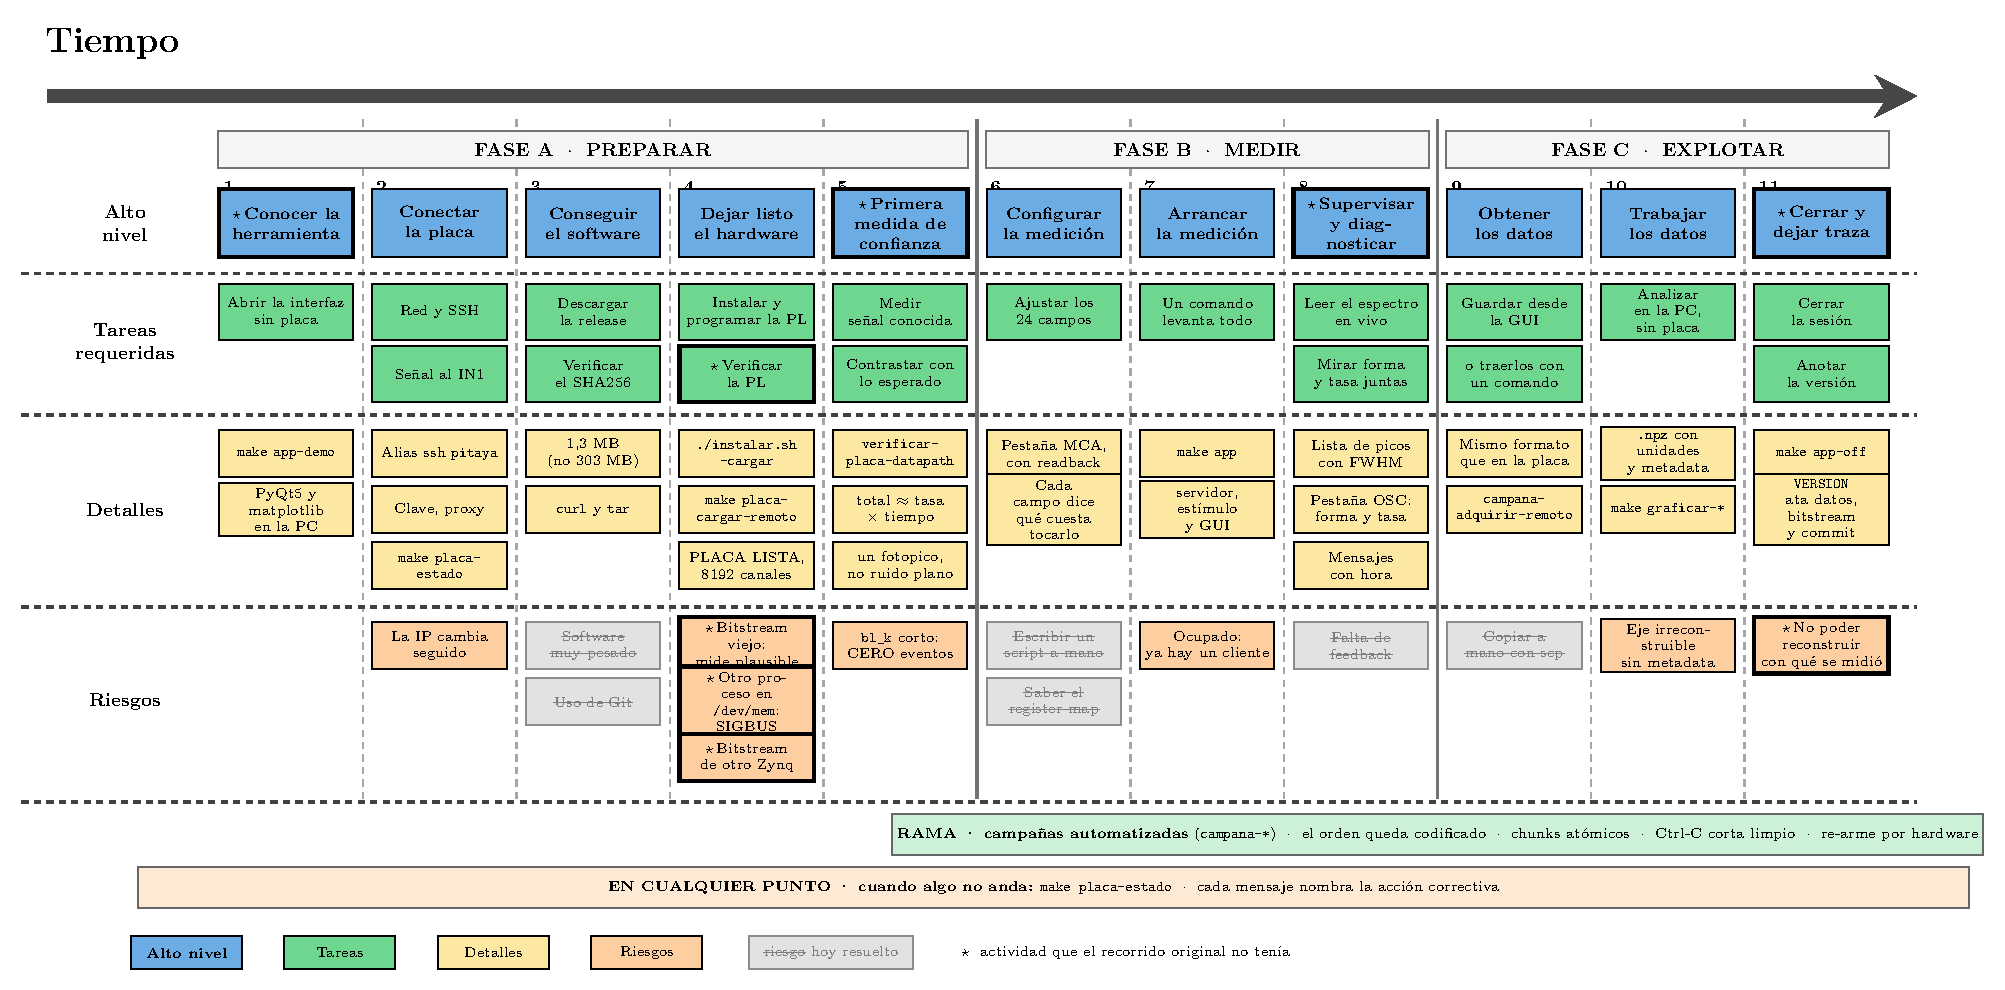
\includegraphics[width=\textwidth]{recorrido_del_usuario.pdf}
%             (es una lámina apaisada; en un documento a una columna conviene
%              \includegraphics[angle=90,height=\textheight]{...})
%
\documentclass[border=10pt,tikz]{standalone}
\usepackage[utf8]{inputenc}
\usepackage[T1]{fontenc}
\usepackage{lmodern}
\usepackage[normalem]{ulem}
\usetikzlibrary{arrows.meta,positioning,calc}

% ---------------------------------------------------------------- colores ---
\definecolor{azul}{RGB}{108,172,228}
\definecolor{verde}{RGB}{110,214,142}
\definecolor{amarillo}{RGB}{252,232,160}
\definecolor{naranja}{RGB}{252,206,160}
\definecolor{grisr}{RGB}{226,226,226}
\definecolor{fase}{RGB}{245,245,245}

% ---------------------------------------------------------------- estilos ---
\tikzset{
  caja/.style   = {draw=black, line width=0.5pt, align=center, inner sep=2.5pt},
  alto/.style   = {caja, fill=azul,     text width=2.1cm, minimum height=1.15cm,
                   font=\footnotesize\bfseries},
  tarea/.style  = {caja, fill=verde,    text width=2.1cm, minimum height=0.95cm,
                   font=\scriptsize},
  detalle/.style= {caja, fill=amarillo, text width=2.1cm, minimum height=0.80cm,
                   font=\scriptsize},
  riesgo/.style = {caja, fill=naranja,  text width=2.1cm, minimum height=0.80cm,
                   font=\scriptsize},
  viejo/.style  = {caja, fill=grisr, draw=black!45, text=black!50,
                   text width=2.1cm, minimum height=0.80cm, font=\scriptsize},
  nuevo/.style  = {line width=1.6pt},
  banda/.style  = {caja, fill=fase, draw=black!55, minimum height=0.62cm,
                   font=\small\bfseries},
  rama/.style   = {caja, fill=verde!35, draw=black!60, minimum height=0.70cm,
                   font=\scriptsize},
  trans/.style  = {caja, fill=naranja!45, draw=black!60, minimum height=0.70cm,
                   font=\scriptsize},
  carril/.style = {font=\small\bfseries, align=center, text width=2.1cm},
  num/.style    = {font=\small\bfseries, anchor=west},
  sepcol/.style = {black!35, dashed, line width=0.7pt},
  sepfase/.style= {black!55, line width=1.1pt},
  sepcarril/.style = {black!75, dashed, line width=1.1pt},
}

% comando en monoespaciado, compacto
\newcommand{\cmd}[1]{{\ttfamily\scriptsize #1}}
% riesgo del recorrido anterior, hoy resuelto
\newcommand{\res}[1]{\sout{#1}}
% marca de actividad que el recorrido original no tenía
\newcommand{\nv}{$\star$\,}

% ----------------------------------------------------------- coordenadas ----
\def\yalto{-1.60}
\def\ytA{-3.10}  \def\ytB{-4.15}
\def\ydA{-5.50}  \def\ydB{-6.45}  \def\ydC{-7.40}
\def\yrA{-8.75}  \def\yrB{-9.70}  \def\yrC{-10.65}

\begin{document}
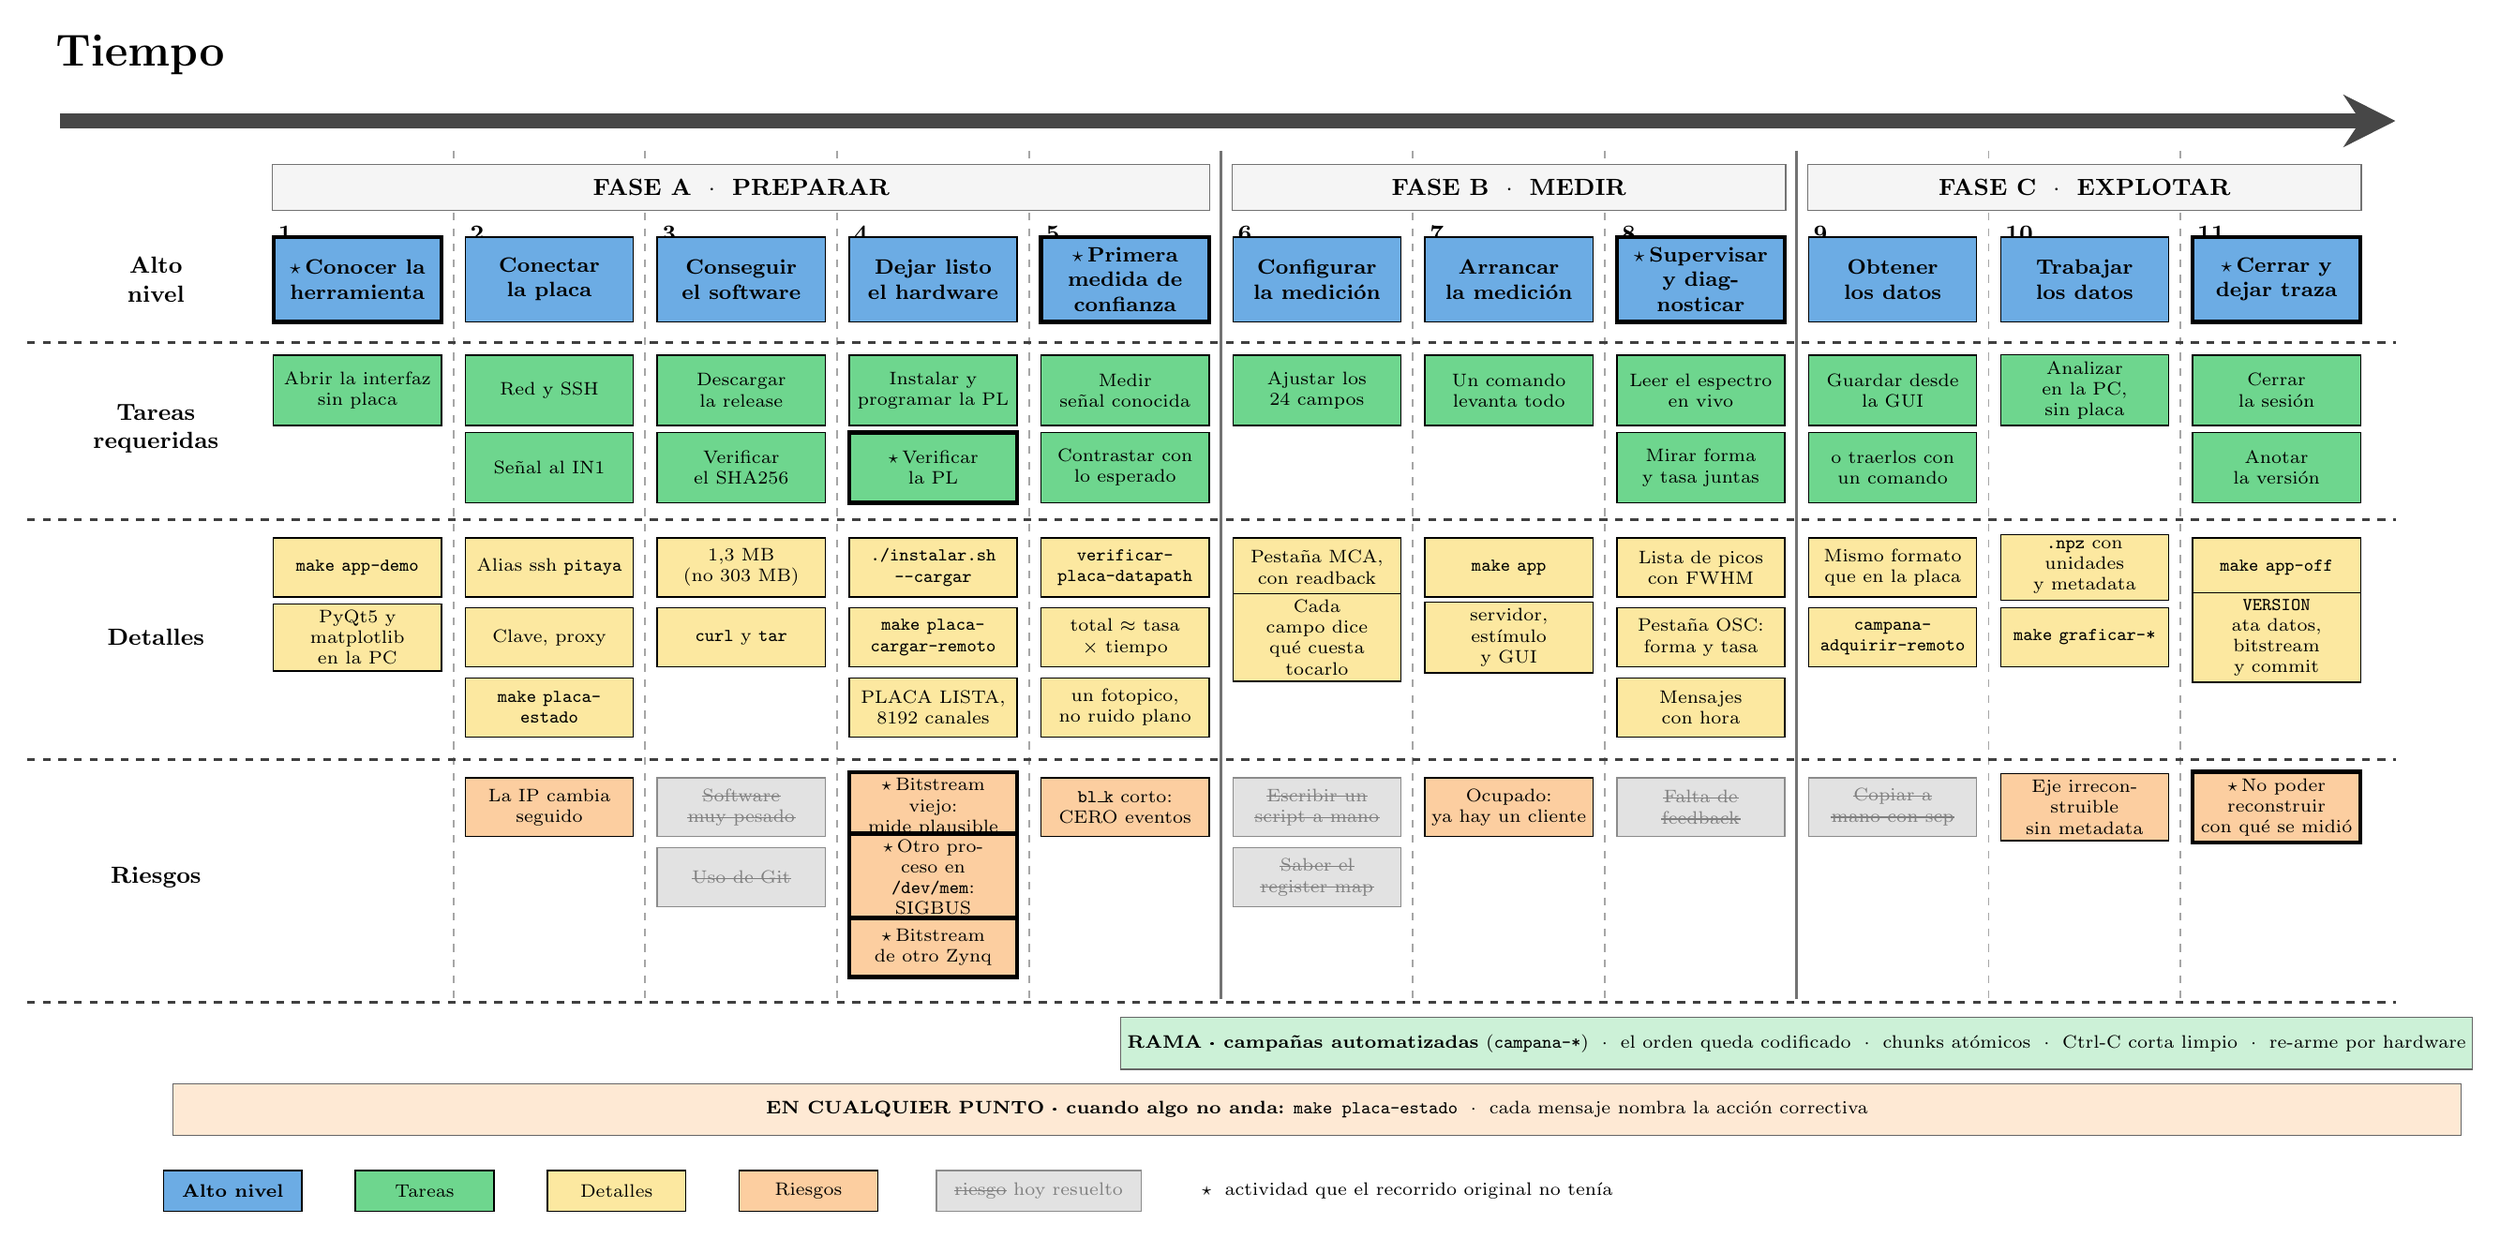
\begin{tikzpicture}[x=2.6cm, y=1cm]

% ===================================================== flecha del tiempo ====
\node[font=\LARGE\bfseries, anchor=west] at (-0.62,1.45) {Tiempo};
\draw[-{Stealth[length=7mm,width=7mm]}, line width=6pt, black!72]
      (-0.55,0.55) -- (11.62,0.55);

% ===================================================== separadores =========
\foreach \i in {1,2,3,4,6,7,9,10}
  \draw[sepcol] (\i+0.5,0.15) -- (\i+0.5,-11.35);
\draw[sepfase] (5.5,0.15) -- (5.5,-11.35);
\draw[sepfase] (8.5,0.15) -- (8.5,-11.35);

\foreach \y in {-2.45,-4.85,-8.10,-11.40}
  \draw[sepcarril] (-0.72,\y) -- (11.62,\y);

% ===================================================== bandas de fase ======
\node[banda, minimum width=12.7cm] at (3,-0.35)  {FASE A \;$\cdot$\; PREPARAR};
\node[banda, minimum width=7.5cm]  at (7,-0.35)  {FASE B \;$\cdot$\; MEDIR};
\node[banda, minimum width=7.5cm]  at (10,-0.35) {FASE C \;$\cdot$\; EXPLOTAR};

% ===================================================== etiquetas de carril ==
\node[carril] at (-0.05,\yalto) {Alto\\nivel};
\node[carril] at (-0.05,-3.62)  {Tareas\\requeridas};
\node[carril] at (-0.05,-6.45)  {Detalles};
\node[carril] at (-0.05,-9.70)  {Riesgos};

% ===================================================== numeración ==========
\foreach \i/\n in {1/1.,2/2.,3/3.,4/4.,5/5.,6/6.,7/7.,8/8.,9/9.,10/10.,11/11.}
  \node[num] at (\i-0.46,-0.98) {\n};

% ======================================================================= 1 ==
\node[alto, nuevo]  at (1,\yalto) {\nv Conocer la herramienta};
\node[tarea] at (1,\ytA) {Abrir la interfaz\\sin placa};
\node[detalle] at (1,\ydA) {\cmd{make app-demo}};
\node[detalle] at (1,\ydB) {PyQt5 y matplotlib\\en la PC};

% ======================================================================= 2 ==
\node[alto]  at (2,\yalto) {Conectar\\la placa};
\node[tarea] at (2,\ytA) {Red y SSH};
\node[tarea] at (2,\ytB) {Señal al IN1};
\node[detalle] at (2,\ydA) {Alias ssh \cmd{pitaya}};
\node[detalle] at (2,\ydB) {Clave, proxy};
\node[detalle] at (2,\ydC) {\cmd{make placa-}\\\cmd{estado}};
\node[riesgo] at (2,\yrA) {La IP cambia\\seguido};

% ======================================================================= 3 ==
\node[alto]  at (3,\yalto) {Conseguir\\el software};
\node[tarea] at (3,\ytA) {Descargar\\la release};
\node[tarea] at (3,\ytB) {Verificar\\el SHA256};
\node[detalle] at (3,\ydA) {1,3 MB\\(no 303 MB)};
\node[detalle] at (3,\ydB) {\cmd{curl} y \cmd{tar}};
\node[viejo] at (3,\yrA) {\res{Software muy pesado}};
\node[viejo] at (3,\yrB) {\res{Uso de Git}};

% ======================================================================= 4 ==
\node[alto]  at (4,\yalto) {Dejar listo\\el hardware};
\node[tarea] at (4,\ytA) {Instalar y\\programar la PL};
\node[tarea, nuevo] at (4,\ytB) {\nv Verificar\\la PL};
\node[detalle] at (4,\ydA) {\cmd{./instalar.sh}\\\cmd{--cargar}};
\node[detalle] at (4,\ydB) {\cmd{make placa-}\\\cmd{cargar-remoto}};
\node[detalle] at (4,\ydC) {PLACA LISTA,\\8192 canales};
\node[riesgo, nuevo] at (4,\yrA) {\nv Bitstream viejo:\\mide plausible};
\node[riesgo, nuevo] at (4,\yrB) {\nv Otro proceso en\\\cmd{/dev/mem}: SIGBUS};
\node[riesgo, nuevo] at (4,\yrC) {\nv Bitstream\\de otro Zynq};

% ======================================================================= 5 ==
\node[alto, nuevo]  at (5,\yalto) {\nv Primera medida de confianza};
\node[tarea] at (5,\ytA) {Medir\\señal conocida};
\node[tarea] at (5,\ytB) {Contrastar con\\lo esperado};
\node[detalle] at (5,\ydA) {\cmd{verificar-}\\\cmd{placa-datapath}};
\node[detalle] at (5,\ydB) {total $\approx$ tasa $\times$ tiempo};
\node[detalle] at (5,\ydC) {un fotopico,\\no ruido plano};
\node[riesgo] at (5,\yrA) {\cmd{bl\_k} corto:\\CERO eventos};

% ======================================================================= 6 ==
\node[alto]  at (6,\yalto) {Configurar\\la medición};
\node[tarea] at (6,\ytA) {Ajustar los\\24 campos};
\node[detalle] at (6,\ydA) {Pestaña MCA,\\con readback};
\node[detalle] at (6,\ydB) {Cada campo dice\\qué cuesta tocarlo};
\node[viejo] at (6,\yrA) {\res{Escribir un script a mano}};
\node[viejo] at (6,\yrB) {\res{Saber el register map}};

% ======================================================================= 7 ==
\node[alto]  at (7,\yalto) {Arrancar\\la medición};
\node[tarea] at (7,\ytA) {Un comando\\levanta todo};
\node[detalle] at (7,\ydA) {\cmd{make app}};
\node[detalle] at (7,\ydB) {servidor, estímulo\\y GUI};
\node[riesgo] at (7,\yrA) {Ocupado:\\ya hay un cliente};

% ======================================================================= 8 ==
\node[alto, nuevo]  at (8,\yalto) {\nv Supervisar y diagnosticar};
\node[tarea] at (8,\ytA) {Leer el espectro\\en vivo};
\node[tarea] at (8,\ytB) {Mirar forma\\y tasa juntas};
\node[detalle] at (8,\ydA) {Lista de picos\\con FWHM};
\node[detalle] at (8,\ydB) {Pestaña OSC:\\forma y tasa};
\node[detalle] at (8,\ydC) {Mensajes\\con hora};
\node[viejo] at (8,\yrA) {\res{Falta de feedback}};

% ======================================================================= 9 ==
\node[alto]  at (9,\yalto) {Obtener\\los datos};
\node[tarea] at (9,\ytA) {Guardar desde\\la GUI};
\node[tarea] at (9,\ytB) {o traerlos con\\un comando};
\node[detalle] at (9,\ydA) {Mismo formato\\que en la placa};
\node[detalle] at (9,\ydB) {\cmd{campana-}\\\cmd{adquirir-remoto}};
\node[viejo] at (9,\yrA) {\res{Copiar a mano con scp}};

% ====================================================================== 10 ==
\node[alto]  at (10,\yalto) {Trabajar\\los datos};
\node[tarea] at (10,\ytA) {Analizar en la PC,\\sin placa};
\node[detalle] at (10,\ydA) {\cmd{.npz} con unidades\\y metadata};
\node[detalle] at (10,\ydB) {\cmd{make graficar-*}};
\node[riesgo] at (10,\yrA) {Eje irreconstruible\\sin metadata};

% ====================================================================== 11 ==
\node[alto, nuevo]  at (11,\yalto) {\nv Cerrar y dejar traza};
\node[tarea] at (11,\ytA) {Cerrar\\la sesión};
\node[tarea] at (11,\ytB) {Anotar\\la versión};
\node[detalle] at (11,\ydA) {\cmd{make app-off}};
\node[detalle] at (11,\ydB) {\cmd{VERSION} ata datos,\\bitstream y commit};
\node[riesgo, nuevo] at (11,\yrA) {\nv No poder reconstruir\\con qué se midió};

% ================================================= rama y banda transversal =
\node[rama, minimum width=15.3cm] at (8.5,-11.95)
  {\textbf{RAMA · campañas automatizadas} (\cmd{campana-*}) \;$\cdot$\;
   el orden queda codificado \;$\cdot$\; chunks atómicos \;$\cdot$\;
   Ctrl-C corta limpio \;$\cdot$\; re-arme por hardware};

\node[trans, minimum width=31.0cm] at (6,-12.85)
  {\textbf{EN CUALQUIER PUNTO · cuando algo no anda:} \cmd{make placa-estado}
   \;$\cdot$\; cada mensaje nombra la acción correctiva};

% ================================================================= leyenda ==
\node[alto,    minimum height=0.55cm, text width=1.7cm, font=\scriptsize\bfseries]
      at (0.35,-13.95) {Alto nivel};
\node[tarea,   minimum height=0.55cm, text width=1.7cm] at (1.35,-13.95) {Tareas};
\node[detalle, minimum height=0.55cm, text width=1.7cm] at (2.35,-13.95) {Detalles};
\node[riesgo,  minimum height=0.55cm, text width=1.7cm] at (3.35,-13.95) {Riesgos};
\node[viejo,   minimum height=0.55cm, text width=2.6cm] at (4.55,-13.95)
      {\res{riesgo} hoy resuelto};
\node[font=\scriptsize, anchor=west] at (5.35,-13.95)
      {$\star$\; actividad que el recorrido original no tenía};

\end{tikzpicture}
\end{document}
